\section{Durchführung}
\label{sec:Durchführung}

\begin{figure}[H]\label{fig:waermepumpe}
    \centering
    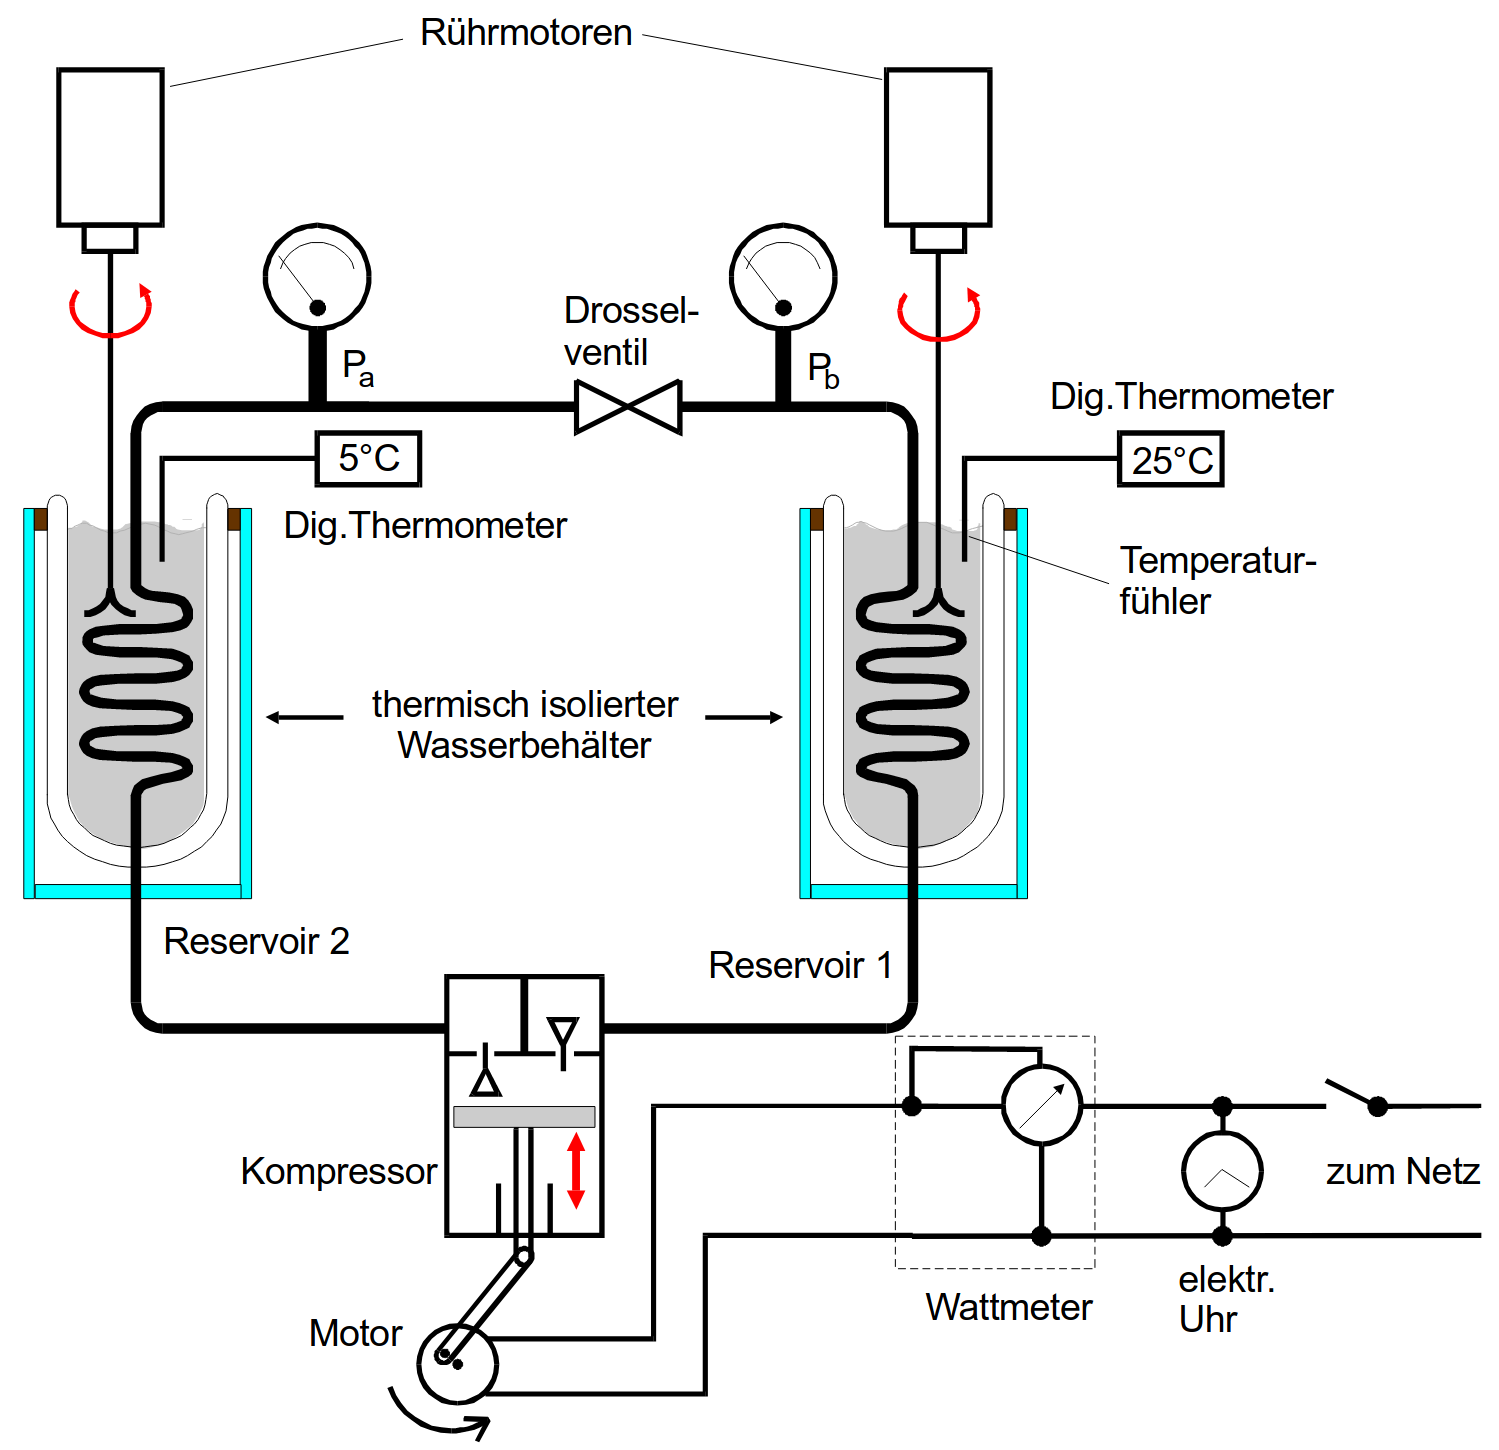
\includegraphics[width=1\textwidth]{content/Aufbau_Waermepumpe.png}
    \caption{Aufbau der Wärmepumpe\protect\footnotemark}
\end{figure}
\footnotetext{Bild entnommen aus Versuchsanleitung V206: Die Wärmepumpe}
%vielleicht sollten wir eine andere Grafik nehmen oder diese hier nochmal bearbeiten weil pa, pb, T1 und T2 bei uns 
%genau gegenteilig benannt sind 

Die Wärmepumpe besteht aus zwei thermisch isolierten, wassergefüllten Reservoiren. Beide Reservoire sind jeweils an ein digitales
Thermometer angeschlossen. Sie sind verbunden durch ein mit $\ce{Cl2F2C}$ gefülltes Kupferrohr. Mit einem Kompressor wird wird 
ein Kreislauf erzeugt. Durch ein Drosselventil D wird ein Druckunterschied mithilfe eines hohen Strömungswiederstand erzeugt. Auf beiden 
Kreislaufseiten ist ein Druckmesser angebracht, mit ihnen können $p_a$ und $p_b$ gemessen werden. Durch den hohen Druck $p_b$
verflüssigt sich das Gas und gibt dadurch Energie an das Reservoir $T_1$. Vor dem Drosselventil wird das Medium durch einen
"Reiniger"  R von Gasbläschen befreit um so eine konstante Zufuhr zum Ventil zu gewährleisten. Um das Wasser in den beiden Reservoiren
gleichmäßig zu erwärmen, werden beide für die Versuchsdauer konstant durchgerührt. Es wird eine Stoppuhr verwendet um die Zeitintervalle zu messen.\\

Für das Experiment werden die Werte der beiden Thermometer, der beiden Druckmesser und die Leistungsaufnahme des Kompressors aufgezeichnet.
Die 5 Messgrößen werden alle 60 Sekunden festgehalten. Das Ablesen erfolgt zyklisch in immer gleicher Reihenfolge: 
$T_2 → T_1 → p_a → p_b → N$

\newpage